\documentclass[]{elsarticle} %review=doublespace preprint=single 5p=2 column
%%% Begin My package additions %%%%%%%%%%%%%%%%%%%
\usepackage[hyphens]{url}

  \journal{Global Health Research and Policy - Thematic Series: Universal Health Coverage} % Sets Journal name


\usepackage{lineno} % add
\providecommand{\tightlist}{%
  \setlength{\itemsep}{0pt}\setlength{\parskip}{0pt}}

\bibliographystyle{elsarticle-harv}
\biboptions{sort&compress} % For natbib
\usepackage{graphicx}
\usepackage{booktabs} % book-quality tables
%%%%%%%%%%%%%%%% end my additions to header

\usepackage[T1]{fontenc}
\usepackage{lmodern}
\usepackage{amssymb,amsmath}
\usepackage{ifxetex,ifluatex}
\usepackage{fixltx2e} % provides \textsubscript
% use upquote if available, for straight quotes in verbatim environments
\IfFileExists{upquote.sty}{\usepackage{upquote}}{}
\ifnum 0\ifxetex 1\fi\ifluatex 1\fi=0 % if pdftex
  \usepackage[utf8]{inputenc}
\else % if luatex or xelatex
  \usepackage{fontspec}
  \ifxetex
    \usepackage{xltxtra,xunicode}
  \fi
  \defaultfontfeatures{Mapping=tex-text,Scale=MatchLowercase}
  \newcommand{\euro}{€}
\fi
% use microtype if available
\IfFileExists{microtype.sty}{\usepackage{microtype}}{}
\usepackage[left=3cm,right=3cm,top=3cm,bottom=3cm]{geometry}
\usepackage{longtable}
\usepackage{graphicx}
% We will generate all images so they have a width \maxwidth. This means
% that they will get their normal width if they fit onto the page, but
% are scaled down if they would overflow the margins.
\makeatletter
\def\maxwidth{\ifdim\Gin@nat@width>\linewidth\linewidth
\else\Gin@nat@width\fi}
\makeatother
\let\Oldincludegraphics\includegraphics
\renewcommand{\includegraphics}[1]{\Oldincludegraphics[width=\maxwidth]{#1}}
\ifxetex
  \usepackage[setpagesize=false, % page size defined by xetex
              unicode=false, % unicode breaks when used with xetex
              xetex]{hyperref}
\else
  \usepackage[unicode=true]{hyperref}
\fi
\hypersetup{breaklinks=true,
            bookmarks=true,
            pdfauthor={},
            pdftitle={Association between compulsory health insurance and life expectency in 184 countries: A retrospective longitudinal study},
            colorlinks=true,
            urlcolor=blue,
            linkcolor=blue,
            pdfborder={0 0 0}}
\urlstyle{same}  % don't use monospace font for urls

\setcounter{secnumdepth}{5}
% Pandoc toggle for numbering sections (defaults to be off)
% Pandoc header
\usepackage{soulutf8}
\usepackage{color}
\usepackage{float}
\usepackage{booktabs}
\usepackage{lscape}
\usepackage{setspace}
\usepackage{dcolumn}



\begin{document}
\begin{frontmatter}

  \title{Association between compulsory health insurance and life expectency in 184 countries: A retrospective longitudinal study}
    \author[SLU]{Miao Cai}
   \ead{miao.cai@slu.edu} 
  
    \author[SLU]{Asabe Garba}
   \ead{asabe.garba@slu.edu} 
  
    \author[WHU]{Xin Li}
   \ead{xl60@iu.edu} 
  
    \author[SCU]{Xiaojun Lin\corref{c1}}
   \ead{xjlin@hust.edu.cn} 
   \cortext[c1]{Corresponding Author}
    \author[SLU]{Ziqi Peng}
   \ead{ziqi.peng@slu.edu} 
  
      \address[SLU]{College for Public Health and Social Justice, Saint Louis University, Saint Louis, MO, 63108}
    \address[SCU]{West China School of Public Health, Sichuan University, Chengdu, Sichuan, China, 610044}
    \address[WHU]{School of Information Management, Wuhan University, Wuhan, Hubei, China, 430072}
  
  \begin{abstract}
  This is the abstract.
  
  It consists of two paragraphs.
  \end{abstract}
  
 \end{frontmatter}

\newcommand{\blandscape}{\begin{landscape}}
\newcommand{\elandscape}{\end{landscape}}
\doublespacing

\hypertarget{introduction}{%
\section{Introduction}\label{introduction}}

\hl{compulsory health insurance and life expectancy.}

In 2010, approximately 1.2 billion people still live in extreme poverty in the world {[}\protect\hyperlink{ref-olinto2013state}{1}{]}.
Poverty is the primary cause of ill-health and loss of life expectancy with exposure to risky environment and insufficient access to health care service {[}\protect\hyperlink{ref-world2001dying}{2}{]}.
To decrease the share of out-of-pocket spending and ensure access to health care among the economically disadvantaged population, health care insurance coverage and prepayment schemes are widely established in health systems around the world {[}\protect\hyperlink{ref-wagstaff2018progress}{3}{]}.
In developing countries, compulsory health insurance is widely introduced as an effective tool to concentrate resources in the health sector and provide needed medical service to the low-income households {[}\protect\hyperlink{ref-abel1992health}{4}--\protect\hyperlink{ref-ensor1999developing}{7}{]}.

In most countries, compulsory health insurance and governmental schemes are the main sources of health care expenditure {[}\protect\hyperlink{ref-healthglance2017}{8}{]}.

\hypertarget{methods}{%
\section{Methods}\label{methods}}

\hypertarget{data-source}{%
\subsection{Data source}\label{data-source}}

We extracted country level data from the Global Health Expenditure Database on the World Health Organization (WHO) website {[}\protect\hyperlink{ref-WHOdata}{9}{]}.
This database provides detailed comparable health expenditure data in around 190 countries from 2000 to 2016.
These health expenditure variables include current health expenditure (CHE) decomposition: domestic government health expenditure, private health expenditure, and out-of-pocket (OOP) payment as percent of CHE;
financing arrangements decomposition: compulsory financing arrangements, government financing arrangements, compulsory health insurance, household OOP payment as percent of CHE; CHE and government health expenditure as percent of gross domestic product (GDP).

Besided country specific decomposed health expenditure and financing arrangements, we also extracted life expectancy, GDP, and population data between 2000 and 2016 in the listed countries from the World Bank Open Data {[}\protect\hyperlink{ref-worldbank}{10}{]}.
Both databases are publicly available, with downloadable comma-separated values or Microsoft Excel files provided on the WHO website.
The two databases were then merged according to two common keys, country name and year.

\hypertarget{variable-selection}{%
\subsection{Variable selection}\label{variable-selection}}

We considered life expectancy at birth in a country in a specific year at the outcome variable in this study.
It reflects the overll mortality level of all age groups in a country in a given year.
Life expectancy is one of the most widely used measure of mortality and burden of disease in previous literature {[}\protect\hyperlink{ref-lee2012effect}{11}--\protect\hyperlink{ref-mathers2015causes}{14}{]}.

We included three key sets of explanatory variables to predict life expectancy in the 184 countries over time.
Country level general characteristics included population (in millions), year (2000 to 2015), and GDP (in billions).
The GDP data were reported in constant 2010 prices, which were adjusted for the effects of price inflation {[}\protect\hyperlink{ref-worldbankconstant}{15}{]}.
Current health expenditure (CHE) and government health expenditure (GGHE-D) as percent of GDP were used to account for the investment in healthcare in a country.
Compulsory financing arrangements and compulsory health insurance as percent of the CHE were included to account for different sources of financing arrangements.
Private health expenditure and OOP payment as percent of the CHE were two sources healthcare expenditure.
These percents varied in the range of 0 and 100.

\hypertarget{statistical-analyses}{%
\subsection{Statistical Analyses}\label{statistical-analyses}}

Observations with missing data in either the dependent variable or any of the explanatory variables were excluded, and we ended up with 2,975 complete observations (91\% of the original data) from 184 countries.
Since only 166 of the 184 countries (90.2\%) had complete data in the sixteen-year period (2000 to 2016), our empirical analysis relied on an unbalanaced country-level panel data.
Among the 184 sample countries, there were 49 in African Region, 35 in Region of the America, 19 in South-East Asia Region, 51 in European Region, 10 in Eastern Mediterranean Region and 23 in Western Pacific Region {[}\protect\hyperlink{ref-WHOregion}{16}{]}.

We estimated the association between compulsory health insurance and life expectancy among the 183 countries using an ordinary least square model, accounting for all the covariates and time trend fixed-effects.
Since high and low income countries can be characterized by different patterns of life expectancy and health financing schemes, we further conducted stratified analyses among the four income category countries to allow for potentially different patterns of association between compulsory health insurance and life expectancy among the 183 countries.
Our main hypothesis is that compulsory health insurance is positively associated with life expectancy.

We reported point and interval estimates (95\% confidence intervals, 95\% CI), as well as the significance of all independent variables.
A p-value less than 0.05 is viewed as statistically significant.
All data cleaning, visualization, statistical modelling, and reporting were performed using statistical computing and graphics environment R, version 3.5.3 {[}\protect\hyperlink{ref-R353}{17}{]}.
In an effort to promote reproducible research, we have created a public GitHub repository to store all the data and R code we used to write this paper.
Interested readers can find them at \url{https://github.com/caimiao0714/GHRP-UHC}.

\hypertarget{results}{%
\section{Results}\label{results}}

\hypertarget{characteristics-of-the-countries-by-income-group}{%
\subsection{Characteristics of the countries by income group}\label{characteristics-of-the-countries-by-income-group}}

\begin{table}[t]

\caption{\label{tab:descriptive}Characteristics of the 184 countries by income group, 2000 - 2016}
\centering
\resizebox{\linewidth}{!}{
\begin{tabular}{lllll}
\toprule
  & Low & Low-Mid & Up-Mid & High\\
\midrule
N & 459 & 830 & 826 & 860\\
Life Expectancy & 56.65 (5.59) & 65.45 (7.26) & 71.22 (5.71) & 77.82 (3.35)\\
Current health expenditure as percent of GDP & 6.15 (2.46) & 5.36 (2.35) & 5.74 (2.15) & 7.21 (2.70)\\
Government Health Expenditure as percent of GDP & 1.40 (0.74) & 2.26 (1.66) & 3.18 (1.64) & 5.09 (2.15)\\
Private health expenditure as percent CHE & 49.91 (18.30) & 47.83 (22.12) & 42.65 (17.53) & 29.39 (12.74)\\
\addlinespace
Out-of-pocket payment as percent of CHE & 44.73 (18.82) & 43.37 (21.81) & 35.00 (17.77) & 22.00 (10.76)\\
Compulsory financing arrangements as percent of CHE & 36.18 (14.99) & 46.49 (21.04) & 55.40 (17.48) & 66.01 (20.50)\\
Compulsory health insurance as percent of CHE & 1.35 (2.53) & 6.58 (9.78) & 18.06 (22.52) & 23.53 (29.31)\\
Population (millions) & 17.71 (19.03) & 54.24 (172.60) & 48.99 (188.88) & 22.34 (47.24)\\
GDP & 0.90 (0.86) & 8.54 (24.51) & 28.61 (89.20) & 86.51 (223.73)\\
\bottomrule
\end{tabular}}
\end{table}

Table \ref{tab:descriptive} presents the characteristics of the study countries stratified by income group. Consistent with Figure 1, high income countries had the highest average life expectancy, followed by up-mid, low-mid, and low income countries. With regard to healthcare expenditure, it appeared that lower income countries had less government health expenditure as percent of GDP, more private health expenditure and OOP payments as percent of GDP, compared to higher income countries. In terms of financing arrangement, higher income countries had higher percent of compulsory financing arrangements and compulsory health insurance as percent of current health expenditure. Compared to low-mid and up-mid income countries, high and low income countries had less population but more current health expenditure as percent of GDP.

\hl{This is not a panel data. Are you sure that 139 countries from 2000 to 2015 were included in Figure 1? It seemed that over 170 countries were included; Data from 2016 was also included in the linear regression models}

\hypertarget{life-expectancy-time-trend-in-different-income-groups}{%
\subsection{Life expectancy time trend in different income groups}\label{life-expectancy-time-trend-in-different-income-groups}}

\begin{figure}
\centering
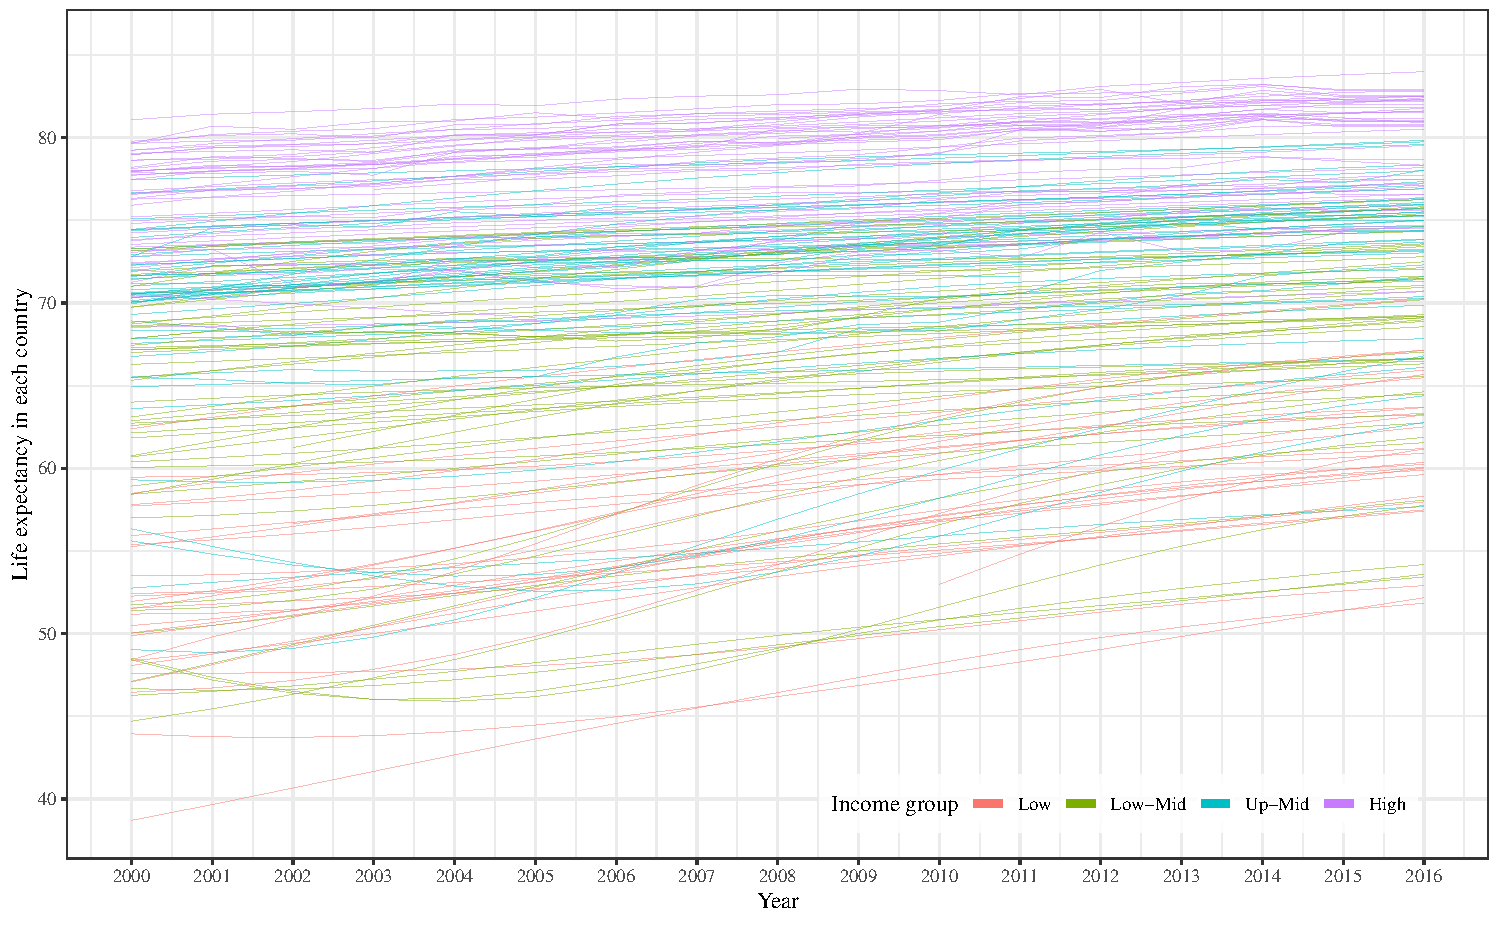
\includegraphics{Figures/fig1.pdf}
\caption{\label{fig:fig1}Life expectancy in 184 countries stratified by country income group, 2000 - 2016}
\end{figure}

Figure \ref{fig:fig1} demonstrates the trend of life expectancy in the 184 countries over the sixteen-year period, with each line represents a country while a color stands for an income category. The life expectancy in the studied countries were generally linearly increasing from 2010 to 2015. The most significant pattern in the plot was that life expectancy was strongly influenced by income group: the high income countries had the highest life expectancy, which increased from about 77 in 2000 to around 80 years old in 2016; the low income countries generally had the lowest life expectancy, which increased from around 50 to about 58 years old. The gap of life expectancy between high and low income countries had narrowed from 2000 to 2016. It was also to be noted that the variance of life expectancy in low and low-mid income countries were much higher than that in up-mid and high income countries.

\hypertarget{potential-life-expectancy-gain-by-compulsory-health-insurance}{%
\subsection{Potential life expectancy gain by compulsory health insurance}\label{potential-life-expectancy-gain-by-compulsory-health-insurance}}

\begin{table}[H] \centering 
  \caption{OLS model predicting life expectancy in 184 countries, 2000 - 2016} 
  \label{poolOLS} 
\begin{tabular}{@{\extracolsep{5pt}}lc} 
\\[-1.8ex]\hline \\[-1.8ex] 
\\[-1.8ex] & Life expectancy \\ 
\hline \\[-1.8ex] 
 Current health expenditure as percent of GDP & 0.162$^{*}$ \\ 
  & (0.026, 0.298) \\ 
  Government health expenditure as percent of GDP & 0.482$^{***}$ \\ 
  & (0.263, 0.702) \\ 
  Private health expenditure as percent CHE & $-$0.154$^{***}$ \\ 
  & ($-$0.186, $-$0.122) \\ 
  Out-of-pocket payment as percent of CHE & 0.174$^{***}$ \\ 
  & (0.146, 0.201) \\ 
  Compulsory financing arrangements as percent of CHE & 0.0003 \\ 
  & ($-$0.016, 0.017) \\ 
  Compulsory health insurance as percent of CHE & 0.035$^{***}$ \\ 
  & (0.025, 0.045) \\ 
  Population (millions) & 0.002$^{**}$ \\ 
  & (0.001, 0.004) \\ 
  GDP & 0.001 \\ 
  & ($-$0.0003, 0.003) \\ 
  Year & 0.301$^{***}$ \\ 
  & (0.263, 0.339) \\ 
  Low income country & $-$19.084$^{***}$ \\ 
  & ($-$19.889, $-$18.280) \\ 
  Low to middle income country & $-$10.936$^{***}$ \\ 
  & ($-$11.539, $-$10.334) \\ 
  Up to middel income country & $-$5.414$^{***}$ \\ 
  & ($-$5.945, $-$4.882) \\ 
  Constant & $-$529.862$^{***}$ \\ 
  & ($-$605.762, $-$453.961) \\ 
 \textit{N} & 2,975 \\ 
R$^{2}$ & 0.695 \\ 
Adjusted R$^{2}$ & 0.694 \\ 
\hline \\[-1.8ex] 
\multicolumn{2}{l}{$^{*}$p $<$ .05; $^{**}$p $<$ .01; $^{***}$p $<$ .001} \\ 
\multicolumn{2}{l}{GDP: Gross Domestic Product} \\ 
\multicolumn{2}{l}{CHE: Current Health Expenditure} \\ 
\end{tabular} 
\end{table}

Table \ref{poolOLS} presents the overall relationship between compulsory health insurance and life expectancy. Controlling for other covariates, one percent increase in compulsory health insurance as percent of CHE was associated with 0.035 years (95\% CI: {[}0.025, 0.045{]}) increase in life expectancy overall.

\hypertarget{potential-life-expectancy-gain-by-compulsory-health-insurance-in-different-income-groups}{%
\subsection{Potential life expectancy gain by compulsory health insurance in different income groups}\label{potential-life-expectancy-gain-by-compulsory-health-insurance-in-different-income-groups}}

Table \ref{stratifiedOLS} presents relationship between compulsory health insurance as percent of CHE and life expectancy in different income group countries. The percent of compulsory health insurance was positive associated with life expectancy among low (\(\beta = 0.224\), 95\% CI: {[}0.055, 0.392{]}), low-mid (\(\beta = 0.243\), 95\% CI: {[}0.195, 0.291{]}), and up-mid income (\(\beta = 0.061\), 95\% CI: {[}0.045, 0.078{]}) countries. However, this association turned out to be negative among high income countries (\(\beta = -0.011\), 95\% CI: {[}-0.018, 0.005{]}), although the effect size was very small.

\begin{landscape}

\begin{table}[!] \centering 
  \caption{OLS model predicting life expectany, 2000 - 2016, stratifeid by country income categories, } 
  \label{stratifiedOLS} 
\begin{tabular}{@{\extracolsep{5pt}}lD{.}{.}{-3} D{.}{.}{-3} D{.}{.}{-3} D{.}{.}{-3} } 
\\[-1.8ex]\hline \\[-1.8ex] 
\\[-1.8ex] & \multicolumn{4}{c}{Life expectancy} \\ 
 & \multicolumn{1}{c}{Low} & \multicolumn{1}{c}{Low-mid} & \multicolumn{1}{c}{Up-mid} & \multicolumn{1}{c}{High} \\ 
\\[-1.8ex] & \multicolumn{1}{c}{Model 1} & \multicolumn{1}{c}{Model 2} & \multicolumn{1}{c}{Model 3} & \multicolumn{1}{c}{Model 4}\\ 
\hline \\[-1.8ex] 
 Current Health Expenditure as percent of GDP & -0.155 & 0.157 & 1.022^{***} & -0.719^{***} \\ 
  & \multicolumn{1}{c}{(-0.377$, $0.067)} & \multicolumn{1}{c}{(-0.122$, $0.436)} & \multicolumn{1}{c}{(0.595$, $1.448)} & \multicolumn{1}{c}{(-1.039$, $-0.399)} \\ 
  Government Health Expenditure as percent of GDP & -0.394 & 0.099 & -0.890^{*} & 1.975^{***} \\ 
  & \multicolumn{1}{c}{(-1.189$, $0.402)} & \multicolumn{1}{c}{(-0.391$, $0.590)} & \multicolumn{1}{c}{(-1.597$, $-0.183)} & \multicolumn{1}{c}{(1.554$, $2.397)} \\ 
  Private Health Expenditure as percent CHE & 0.174^{***} & -0.373^{***} & -0.137^{***} & 0.116^{***} \\ 
  & \multicolumn{1}{c}{(0.087$, $0.262)} & \multicolumn{1}{c}{(-0.469$, $-0.277)} & \multicolumn{1}{c}{(-0.215$, $-0.059)} & \multicolumn{1}{c}{(0.072$, $0.159)} \\ 
  Out-of-pocket payment as percent of CHE & -0.172^{***} & 0.435^{***} & 0.239^{***} & -0.043^{*} \\ 
  & \multicolumn{1}{c}{(-0.254$, $-0.090)} & \multicolumn{1}{c}{(0.349$, $0.520)} & \multicolumn{1}{c}{(0.201$, $0.277)} & \multicolumn{1}{c}{(-0.076$, $-0.010)} \\ 
  Compulsory Financing Arrangements as percent of CHE & -0.024 & 0.054 & 0.148^{***} & 0.002 \\ 
  & \multicolumn{1}{c}{(-0.075$, $0.026)} & \multicolumn{1}{c}{(-0.008$, $0.116)} & \multicolumn{1}{c}{(0.087$, $0.210)} & \multicolumn{1}{c}{(-0.009$, $0.012)} \\ 
  Compulsory health insurance as percent of CHE & 0.224^{**} & 0.243^{***} & 0.061^{***} & -0.011^{***} \\ 
  & \multicolumn{1}{c}{(0.055$, $0.392)} & \multicolumn{1}{c}{(0.195$, $0.291)} & \multicolumn{1}{c}{(0.045$, $0.078)} & \multicolumn{1}{c}{(-0.018$, $-0.005)} \\ 
  Population (millions) & -0.056^{*} & -0.005 & 0.003 & 0.012 \\ 
  & \multicolumn{1}{c}{(-0.100$, $-0.012)} & \multicolumn{1}{c}{(-0.012$, $0.002)} & \multicolumn{1}{c}{(-0.001$, $0.007)} & \multicolumn{1}{c}{(-0.009$, $0.032)} \\ 
  GDP & 2.435^{***} & 0.060^{*} & 0.001 & -0.003 \\ 
  & \multicolumn{1}{c}{(1.427$, $3.444)} & \multicolumn{1}{c}{(0.011$, $0.109)} & \multicolumn{1}{c}{(-0.007$, $0.009)} & \multicolumn{1}{c}{(-0.007$, $0.002)} \\ 
  Year & 0.506^{***} & 0.289^{***} & 0.225^{***} & 0.158^{***} \\ 
  & \multicolumn{1}{c}{(0.409$, $0.602)} & \multicolumn{1}{c}{(0.200$, $0.378)} & \multicolumn{1}{c}{(0.160$, $0.290)} & \multicolumn{1}{c}{(0.122$, $0.195)} \\ 
  Constant & -958.790^{***} & -521.271^{***} & -395.563^{***} & -247.217^{***} \\ 
  & \multicolumn{1}{c}{(-1,152.821$, $-764.759)} & \multicolumn{1}{c}{(-699.343$, $-343.198)} & \multicolumn{1}{c}{(-525.258$, $-265.868)} & \multicolumn{1}{c}{(-319.848$, $-174.585)} \\ 
 \textit{N} & \multicolumn{1}{c}{459} & \multicolumn{1}{c}{830} & \multicolumn{1}{c}{826} & \multicolumn{1}{c}{860} \\ 
R$^{2}$ & \multicolumn{1}{c}{0.391} & \multicolumn{1}{c}{0.304} & \multicolumn{1}{c}{0.385} & \multicolumn{1}{c}{0.465} \\ 
Adjusted R$^{2}$ & \multicolumn{1}{c}{0.379} & \multicolumn{1}{c}{0.296} & \multicolumn{1}{c}{0.378} & \multicolumn{1}{c}{0.460} \\ 
\hline \\[-1.8ex] 
\multicolumn{5}{l}{$^{*}$p $<$ .05; $^{**}$p $<$ .01; $^{***}$p $<$ .001} \\ 
\end{tabular} 
\end{table} 
\end{landscape}

\hypertarget{discussion}{%
\section{Discussion}\label{discussion}}

In this study, we explored the association between compulsory health insurance and life expectancy in 184 countries over 16 years. Our regression models revealed that compulsory health insurance was significantly associated with life expectancy, after adjusting for country level characteristics, health expenditure and other health financing arrangements.

\hypertarget{acknowledgements}{%
\section*{Acknowledgements}\label{acknowledgements}}
\addcontentsline{toc}{section}{Acknowledgements}

We thank the WHO and the World Bank for making data used in this study publicly available for researchers.

\hypertarget{funding}{%
\section*{Funding}\label{funding}}
\addcontentsline{toc}{section}{Funding}

None.

\hypertarget{availability-of-data-and-materials}{%
\section*{Availability of data and materials}\label{availability-of-data-and-materials}}
\addcontentsline{toc}{section}{Availability of data and materials}

All data and associated R code are public available at the GitHub repository \texttt{caimiao0714/GHRP-UHC}, which can be accessed at \url{https://github.com/caimiao0714/GHRP-UHC}.

\hypertarget{references}{%
\section*{References}\label{references}}
\addcontentsline{toc}{section}{References}

\hypertarget{refs}{}
\leavevmode\hypertarget{ref-olinto2013state}{}%
1. Olinto P, Beegle K, Sobrado C, Uematsu H, others. The state of the poor: Where are the poor, where is extreme poverty harder to end, and what is the current profile of the world's poor. Economic Premise. 2013;125:1--8.

\leavevmode\hypertarget{ref-world2001dying}{}%
2. Organization WH, others. Dying for change: Poor people's experience of health and ill-health. 2001.

\leavevmode\hypertarget{ref-wagstaff2018progress}{}%
3. Wagstaff A, Flores G, Smitz M-F, Hsu J, Chepynoga K, Eozenou P. Progress on impoverishing health spending in 122 countries: A retrospective observational study. The Lancet Global Health. 2018;6:e180--92.

\leavevmode\hypertarget{ref-abel1992health}{}%
4. Abel-Smith B. Health insurance in developing countries: lessons from experience. Health policy and Planning. 1992;7:215--26.

\leavevmode\hypertarget{ref-abel1994employer}{}%
5. Abel-Smith B. Employer's willingness to pay: the case for compulsory health insurance in Tanzania. Health Policy and Planning. 1994;9:409--18.

\leavevmode\hypertarget{ref-jowett2003impact}{}%
6. Jowett M, Contoyannis P, Vinh ND. The impact of public voluntary health insurance on private health expenditures in Vietnam. Social science \& medicine. 2003;56:333--42.

\leavevmode\hypertarget{ref-ensor1999developing}{}%
7. Ensor T. Developing health insurance in transitional Asia. Social Science \& Medicine. 1999;48:871--9.

\leavevmode\hypertarget{ref-healthglance2017}{}%
8. OECD. Health at a Glance 2017. 2017. doi:\href{https://doi.org/https://doi.org/https://doi.org/10.1787/health_glance-2017-en}{https://doi.org/https://doi.org/10.1787/health\_glance-2017-en}.

\leavevmode\hypertarget{ref-WHOdata}{}%
9. The World Health Organization. Global Health Expenditure Database. 2016. \url{http://apps.who.int/nha/database/Select/Indicators/en}. Accessed 20 Mar 2019.

\leavevmode\hypertarget{ref-worldbank}{}%
10. The World Bank. World Bank Open Data. 2018. \url{https://data.worldbank.org/}. Accessed 6 Apr 2018.

\leavevmode\hypertarget{ref-lee2012effect}{}%
11. Lee I-M, Shiroma EJ, Lobelo F, Puska P, Blair SN, Katzmarzyk PT, et al. Effect of physical inactivity on major non-communicable diseases worldwide: An analysis of burden of disease and life expectancy. The lancet. 2012;380:219--29.

\leavevmode\hypertarget{ref-salomon2012healthy}{}%
12. Salomon JA, Wang H, Freeman MK, Vos T, Flaxman AD, Lopez AD, et al. Healthy life expectancy for 187 countries, 1990--2010: a systematic analysis for the Global Burden Disease Study 2010. The Lancet. 2012;380:2144--62.

\leavevmode\hypertarget{ref-bennett2015future}{}%
13. Bennett JE, Li G, Foreman K, Best N, Kontis V, Pearson C, et al. The future of life expectancy and life expectancy inequalities in England and Wales: Bayesian spatiotemporal forecasting. The Lancet. 2015;386:163--70.

\leavevmode\hypertarget{ref-mathers2015causes}{}%
14. Mathers CD, Stevens GA, Boerma T, White RA, Tobias MI. Causes of international increases in older age life expectancy. The Lancet. 2015;385:540--8.

\leavevmode\hypertarget{ref-worldbankconstant}{}%
15. The World Bank. What is the difference between current and constant data? 2018. \url{https://datahelpdesk.worldbank.org/knowledgebase/articles/114942-what-is-the-difference-between-current-and-constan}. Accessed 6 Apr 2018.

\leavevmode\hypertarget{ref-WHOregion}{}%
16. The World Health Organization. Definition of regional groupings. 2019. \url{https://www.who.int/healthinfo/global_burden_disease/definition_regions/en/}. Accessed 20 Mar 2019.

\leavevmode\hypertarget{ref-R353}{}%
17. R Core Team. R: A Language and Environment for Statistical Computing. Vienna, Austria: R Foundation for Statistical Computing; 2019. \url{https://www.R-project.org/}.

\end{document}


